На рисунках 
\ref{fig:BPS_Catia_Top}--\ref{fig:BPS_Catia_Front} показана геометрическая модель ``в плане'' гипотетической конструкции БПЛА.


\begin{figure}[H]
\centering
\def\svgwidth{0.9\textwidth}
\input{figures/BPS_Catia_Top.pdf_tex}
\caption{Вид сверху}
\label{fig:BPS_Catia_Top}
\end{figure}

Как видно из рисунков, для данной компоновочной схемы используется крыло большого удлинения величиной $\lambda = todo$. Из рисунков \ref{fig:BPS_Catia_Front},\ref{fig:BPS_Catia_WithoutSkin}, на котором представлена базовая КСС БПЛА, можно видеть, как происходит интеграция корпуса фюзеляжа, крыла и двигателя. 

\begin{figure}[H]
\centering
\input{figures/BPS_Catia_Front.pdf_tex}
%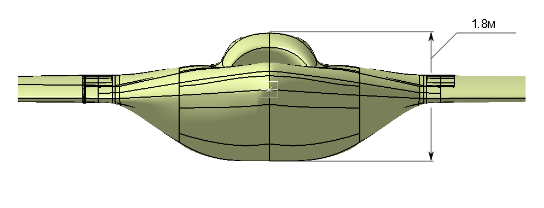
\includegraphics[width=0.8\textwidth]{BPS_Catia_Front}
\caption{Вид фюзеляжа спереди}
\label{fig:BPS_Catia_Front}
\end{figure}

%\begin{figure}[H]
%\centering
%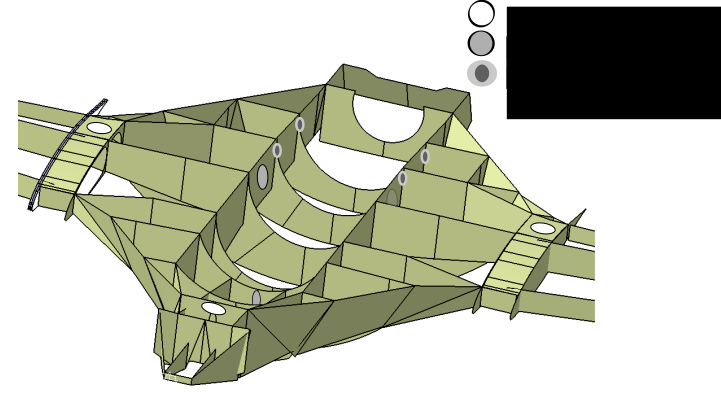
\includegraphics[width=0.8\textwidth]{BPS_Catia_WithoutSkin}
%\caption{Основные рамы корпуса БПЛА}
%\label{fig:BPS_Catia_WithoutSkin}
%\end{figure}

\begin{figure}[H]
\centering
\def\svgwidth{0.9\textwidth}
\input{figures/BPS_Catia_WithoutSkin.pdf_tex}
\caption{Основные рамы корпуса БПЛА}
\label{fig:BPS_Catia_WithoutSkin}
\end{figure}

В модели гипотетической конструкции БПЛА отсутствует вертикальное оперение. Горизонтальное оперение представлено рулем высоты. Механизация крыла состоит из расщепляющихся элеронов на концах крыльев, элевонов на средней части крыла и интерцепторов, расположенных ближе к фюзеляжу. На рисунке \ref{fig:BPS_Catia_Top_WithoutSkin} схематически показаны места крепления основных навесных агрегатов (двигателя) и стоек шасси в виде кругов соответствующей формы. 

Из рисунков видно, что двигатель с воздухозаборником значительно утоплены в конструкцию корпуса и находятся практически в середине (по высоте) фюзеляжа. Как уже отмечалось выше, эта особенность позволяет значительно улучшить малозаметность и аэродинамическое качество самолета (ссылка на отчет), но приводит к необходимости формировать искривленный центроплан. 

Формирование искривленного центроплана сопряжено с большим риском весовых потерь из-за большой величины изгибающего момента в корне крыла, а также из-за наличия сжатых искривленных панелей кессона центроплана. Еще одной проблемой обеспечения прочности корпуса БПЛА является высокая чувствительность параметров управляемости БПЛА к изменению жесткостных характеристик корпуса и особенно зоны стыка крыла с центропланом, где расположены узлы крепления стоек основного шасси. 

%В качестве силовой установки используется один реактивный двигатель, углубленный в конструкцию вместе с воздухозаборником. 
%Места креплений стоек и замков шасси, расположение двигателя и узлов его крепления показаны на Рис. \ref{fig:BPS_Catia_Top_WithoutSkin}. 
Очевидно, что для решения проектировочной задачи необходимо проведение комплексных исследований прочности данной конструкции включая анализ прочности, устойчивости и управляемости в рамках единой прочностной модели всей конструкции гипотетического БПЛА. 



\begin{figure}[H]
\centering
\def\svgwidth{0.9\textwidth}
\input{figures/BPS_Catia_Top_WithoutSkin.pdf_tex}
\caption{Компоновочная схема гипотетической конструкции БПЛА. Вид сверху}
\label{fig:BPS_Catia_Top_WithoutSkin}
\end{figure}
 

На Рис.\ref{fig:BPS_Catia_Top_PartRoles} схематически показаны основные отсеки конструкции БПЛА. 

\begin{figure}[H]
\centering
\def\svgwidth{0.9\textwidth}
\input{figures/BPS_Catia_Top_PartRoles.pdf_tex}
\caption{Компоновочная схема гипотетической конструкции БПЛА с указанием основных отсеков. Вид сверху}
\label{fig:BPS_Catia_Top_PartRoles}
\end{figure}
